\documentclass[a4paper, bibliography=totoc, oneside, 12pt]{scrbook}
\usepackage[american]{babel}
\usepackage{csquotes}
\usepackage[style=apa,sortcites=true,sorting=nyt,backend=biber]{biblatex}
\DeclareLanguageMapping{american}{american-apa}
\addbibresource{bibliography.bib}

\usepackage[inline]{enumitem} % numbered lists
\usepackage{ragged2e} % justification
\usepackage{textcomp}
\usepackage{setspace}
\usepackage{microtype} % fixes line breaks
\usepackage[a4paper, margin=2.5cm, top=3.5cm, bottom=3.5cm]{geometry}
\usepackage[automark, headsepline, singlespacing=true]{scrlayer-scrpage}
\usepackage{varioref}
\usepackage{hyperref}
\usepackage[capitalise]{cleveref}
\usepackage{pdfpages}
\usepackage{epigraph}
\usepackage{xcolor} % http://tex.stackexchange.com/a/150377
\usepackage{listings}
\usepackage{tocbibind}
\usepackage{siunitx}

\linespread{1.25}

\graphicspath{ {./images/} }

\definecolor{linenumbers}{rgb}{0.25, 0.25, 0.25}
\definecolor{linebreakmarker}{rgb}{0.25, 0.25, 0.25}

\lstset{ %
  belowcaptionskip=1\baselineskip{},
  breaklines=true,
  postbreak=\mbox{\textcolor{linebreakmarker}{$\hookrightarrow$}\space},
  captionpos=b,
  numbers=left,
  numbersep=16pt,
  numberstyle=\tiny\color{linenumbers},
  tabsize=2
}

% === actual document === %

\title{Aligning Mental Models and Models Used in Software Development}
\author{Bernhard Mayr}

\clearpairofpagestyles
\ohead*{\pagemark}

\begin{document}

\makeatletter
\begin{titlepage}
   \begin{center}
        Institut für Psychologie\\
        Fakultät für Psychologie und Sportwissenschaften\\
        Leopold--Franzens--Universität Innsbruck
 
        \vspace{4cm}
        \textit{\textbf{\Large {\@title}}}
 
        \vspace{2cm}
        Bachelorarbeit\\
        zur Erlangung des akademischen Grades\\
        Bachelor of Science (B. Sc.)\\
        im Fach Psychologie
 
        \vspace{3cm}
        eingereicht von\\
        \textit{\@author, 11730144}
 
        \vfill
 
        Supervisor: \textit{Univ.-Prof. Dr. Pierre Sachse}\\
        Innsbruck, \textit{\today}
   \end{center}
\end{titlepage}

\frontmatter
\setcounter{page}{2}

\chapter{Acknowledgements}
\chapter{Abstract}
\todo{that's new}
\noindent
Despite of being a human activity, developing software usually does not receive the amount of psychological research needed.
A major difficulty is the huge gap between those two disciplines being the reason for this missing interdisciplinary thinking.
Developing software is way too often reduced to the act of entering commands in a way the computer does what the programmer wants it to do.
In reality a lot of steps happen until software developers can express their ideas in such a clarity that they are able to create an executable and correct program.
Looking at the software development process holistically and applying ideas of cognitive psychology, especially these of mental models, the author of this thesis tries to align the thought process behind creating software closer with the actual technical process of doing it.
This leads to the research question: \emph{Which findings of cognitive and social psychology support the usage of statecharts combined with hole-driven development for enabling better communication in software development processes, or how can these concepts be adapted to closer align to the way the human brain works?}

\vspace{2cm}
\noindent
Keywords: mental models, psychology of programming, statecharts
\chapter{Kurzfassung}
Die Entwicklung von Software ist eine äußerst menschenzentrierte Angelegenheit.
Die Aufmerksamkeit, die ihr die Psychologie dabei schenkt, ist im Gegensatz verschwindend gering, was durchaus am sehr großen Unterschied dieser zwei Wissenschaftsbereiche liegt.
Viel zu oft wird Programmieren auf das reine Erstellen von Quelltexten reduziert oder umgangssprachlich gar als Tippen von Nullen und Einsen bezeichnet.
In Wirklichkeit sind die Prozesse, die zum Erstellen von Software notwendig sind, allerdings wesentlich komplexer und interdisziplinärer.
Das Ziel dieser Arbeit ist die Betrachtung des Softwareentwicklungsprozesses aus der psychologischen Perspektive, wobei der Fokus auf der Erstellung und Weitergabe von mentalen Modellen und gemeinsamem Verständnis liegt.
Die Forschungsfrage lautet daher: \emph{Durch die Kombination von Statecharts und Hole-Driven-Development entsteht eine neue Art und Weise Software zu entwickeln.
Welche Erkenntnisse der Kognitions- und Sozialpsychologie unterstützen diese Kombination bzw. wie kann die Softwareentwicklung so adaptiert werden, dass sie den Prozessen unseres Gehirns ähnelt?}

\vspace{2cm}
\noindent
Keywords: Mentale Modelle, Psychologie der Computerprogrammierung, Statecharts

\tableofcontents
\mainmatter

\chapter{Introduction}
\epigraph{A programmer does not primarily write code; rather, he primarily writes to another programmer about his program solution.}{\textit{Unknown}}
Unfortunately the author of this rather social definition of a programmer's tasks was not handed down, nevertheless the article \textcite{noauthor_what_1967} collected by Don Knuth laid the foundation for human-centered programming.
Reading Peter Naur's influential article \citetitle{naur_programming_1985} written in \citeyear{naur_programming_1985} this human-centered approach to programming seems to be forgotten. Only 18 years later he states that: "[...] much current discussion of programming seems to assume that programming is similar to industrial production, the programmer being regarded as a component of that production, a component that has to be controlled by rules of procedure and which can be replaced easily."
At the same the interdisciplinary research field \emph{Psychology of Programming} originated \autocite{myers_past_2009}, indicating that this mismatch of what programming is and as what it is seen was recognized.


\section{Problem Definition}
\label{sec:problem-definition}
As stated in \textcite{noauthor_what_1967} programming is a communication process.
Even if programming is not seen as a mainly human-centered activity, translating thoughts into a language understood by machines is a form of communication, namely \emph{Human Computer Interaction} (HCI).
As software got more and more complex, the sole activity of programming transitioned to the much broader task of software development.
This process begins with the task of requirements analysis, after aquiring a common understanding in the whole team, those have to be implemented, tested and shipped to the customer \autocite{mayr_projekt_2005}.
Alone this extremely simplified description of software development exhibits the difference to programming.
Comparing this to the Psychology of Programming \citeauthor{curtis_psychology_1990} stated: "The fact that this field is usually referred to as the 'psychology of programming' rather than the 'psychology of software development' reflects its primary orientation to the coding phenomena." \autocite[267]{curtis_psychology_1990}.

In modern frameworks the process of software development happens iteratively and incrementally \autocite{mayr_projekt_2005} which means that user feedback is constantly incorporated into the development cycle.
New requirements arise or existing ones have to be adapted, in either case the software under development has to be adapted.
The basis for this adoption is communication, a human factor, that does not come without difficulties (see \cref{sec:characteristics-of-software-development-processes}).
As \citeauthor{curtis_psychology_1990} state in their essay \textcite{curtis_psychology_1990} mainly organizational processes characterize software development.

\emph{Source of truth} is a saying commonly used in software development for the place where something is defined.
Good software design favors a single source of truth, because then changing stuff means changing it only in one place.
Applying this idea to the whole software development process the single source of truth is the actual source code.
No matter what a requirements document defines or what the user documentation states, if those are not in sync with the source code, they "lose", the code \emph{speaks the real truth}.

So why not take \citeauthor{schraube_ich_2012}'s ideas \autocite{schraube_ich_2012} that technology influences people the same way they influence technology and apply those in a way that establishes a technology-based rethinking process inducing a change in organizational processes.


\section{Research Question}
The problem as previously described is usually not perceived as such one in the software development industry, it's just the characteristics of software development processes and inherently caused by the way software is currently produced.
In Bret Victor's words this \emph{problem} might rather be stated as a \emph{principle} of how software development might look like \autocite{victor_inventing_2012}.
The upcoming ideas emerged from the authors psychology internship at the company Innerspace GmbH in Wattens, Austria.
Usually employed as a software architect the author switched perspectives for two months and studied the software development process from an external view.
The company Innerspace creates virtual reality trainings for pharmaceutical companies.
One main difference to traditional web or desktop application development is the amount of interdisciplinary people involved in the process of creating virtual reality trainings.
In addition to software developers, 3D artists, training designers, narrators and game engineers are needed for content creation.
As stated in \cref{sec:problem-definition} in the end the source code is the actual source of truth.
Because 3D assets, narrations and the training flows are also artifacts of the development process they have to be aligned to this source of truth.

While researching possible technical solutions for the problem of managing state in complex applications like virtual reality trainings the author stumbled upon the rather old concept of \emph{Statecharts} \autocite{harel_statecharts:_1987}. Statecharts are a "visual formalism for complex systems". In more general words this means that Statecharts describe a mathematically proven visual language for creating computer programs. The visual notation is executable and can directly be aligned to a textual notation, which results in the fact, that a written program can be visualized automatically. This visualization combines flowcharts and state diagrams. On top of that this visualization provides simulation capabilities and therefore enables people to visually see and experiment with the logic of the program, without actually using the program. In fact, the program might not even exist at this point, but people can collaboratively design what the program should do. The main hypothesis is that this duality of visualization and executability enables the creation of a common mental model, resulting in a common basis of communication.

To further improve this communication process, the fractal nature of Statecharts (logic can be refined from abstract to concrete) is the perfect fit for hole driven development (see \cref{sec:hole-driven-development}). This relatively new idea of writing computer programs can be compared with a "fill in the blank"-exercise. Instead of having to write a complete program, developers can leave holes for the computer and then ask it to provide help based on mathematical reasoning. Applying this idea at the level of human interaction, the second hypothesis is that introducing holes in Statecharts (enabled by their fractal and composable nature) enables a new way of communicating, defining and refining requirements.

This leads to the research question: \emph{Which findings of cognitive and social psychology support the usage of Statecharts combined with hole driven development for enabling better communication in software development processes, or how can those concepts be adapted to closer align to the way the human brain works?}


% Utilizing the features of Statecharts and hole driven development to align this process closer to how people think might result in a huge productivity boost and take a lot of burden off the people involved in creating software.
\chapter{Technological Foundation}
\label{chap:technological-foundation}
\epigraph{``I became convinced from the start that the notion of a state and a transition to a new state was fundamental to their thinking about the system.''}{\textit{David Harel}}
\noindent
Crossing the interdisciplinary boundaries between programming and psychology needs the definition of the technical concepts that are referenced.
For example knowing what is meant by \emph{state} and \emph{transition} in David Harel's above-mentioned psychological discovery is necessary to understand why this might impact the way people think about systems. 
As stated by \textcite{schraube_ich_2012}, the interaction between a person's psyche and technology is always bidirectional, we get shaped by technology the same way we shape it.

\section{Characteristics of Software Development Processes}
\todo{that's new}
\label{sec:characteristics-of-software-development-processes}
Upon answering the question on how communication in software development processes can be improved using technology, it is important to define these processes, take a quick look at the history and examine the difficulties of changing requirements.

The complex process of software development involves a lot of tasks, stakeholders and uncertainties \autocite{mayr_projekt_2005}.
Being able to plan, organize and control this process, different paradigms of organizing the process of software development were established and improved.
Independent of the software development paradigm, six main phases can be identified, namely: \emph{requirements analysis}, \emph{specification}, \emph{design}, \emph{implementation}, \emph{testing} and \emph{maintenance} \autocite{harel_statecharts:_1987}.
Somehow those phases have to be completed in that order, albeit the paradigms differ in the way the phases are went through, 
The most notable differences are the flexibility in adapting to changing requirements, customer communication, the way phase transitions are handled, how fast the project iterates and how often intermediate results are delivered \autocite{mayr_projekt_2005}.

\subsection{Traditional Paradigms vs. Agile Paradigms}
\todo{that's new}
\label{sub:traditional-vs-agile}
As described in \textcite{mayr_projekt_2005}, the evolution of software development paradigms underwent a lot of change.
Over time the characteristics changed from rigorous (traditional, heavy and stable) to agile (modern, lean, fragile), with the agile movement based on \textcite{fowler_agile_2000} as the current status quo \autocite{ousterhout_philosophy_2018}.
In comparison to the documentation-heavy traditional paradigms, agile paradigms got rid of documentation overhead, heavily rely on prototyping and follow an iterative-incremental model \autocite{mayr_projekt_2005}.
This iterative-incremental model is characterized by short consecutive development cycles and a high frequency in delivering intermediate products, thus staying in close contact with the customer, making sure that the right product is delivered and requirements are understood correctly \autocite{mayr_projekt_2005}.
Dispensing long requirement analysis and specification phases in favor of a short time to market affects software architecture and design, subsequently complicating the creation of well-architectured, solid software.
\textcite{ousterhout_philosophy_2018} introduces the terms \emph{tactical programming} and \emph{strategic programming}.
While the main focus of tactical programming is to create something that works, the focus of strategic programming is to create something that lasts.
In the end this is a business decision, but the effects it has on software development have a huge impact regarding the design of stable, well-constructed systems \autocite{ousterhout_philosophy_2018}.

\subsection{Requirements Analysis and Changing Requirements}
\label{sub:requirements-analysis}
Requirements are properties that have to be fulfilled by a system \autocite{mayr_projekt_2005}.
Requirements analysis is the process of understanding what the customer needs and translating these to a specification upon which the software program can be built.
It is necessary that these identified requirements can be validated and verified.

As stated in \textcite{mayr_projekt_2005} the difficulties of requirements analysis are often underestimated.
Two of these are of high importance for this thesis.
Requirements analysis is a human-centered communication process.
Analysts have to understand the customer's domain, excel at communication with various stakeholders and create a form of specification that is understood by all participants as well as traceable from the origin of a requirement into the finished product.
As \textcite[265]{curtis_psychology_1990} discovered: ``That is, many projects spen[d] tremendous time rediscovering information that, in many cases, had already been generated by customers, but not transmitted.''
Changing requirements caused by the customer, by competitors or by new market innovations are another big problem for requirements analysis.
As stated by \textcite{mayr_projekt_2005}, requirements analysts' methods and notations should favor an easy way of adapting new and changing requirements.

Even if the analysts' methods can adapt to changing requirements, the difficulty of communication still exists and gets intensified by rapidly changing requirements.
More closely aligning the methods and notations of analysts to those used in the implementation phase can reduce these costly communication problems.
According to Peter Naur the designer's (analyst's in this case) job is not to pass along ``the design'' but to pass on ``the theories'' driving the design \autocite{naur_programming_1985} preventing documentation being an ``auxiliary, secondary product.''

\textcite{leveson_experiences_1991} report an interesting experience on requirements specification while working on an aircraft collision avoidance system called \emph{TCAS II}.
After realizing that the \emph{minimal operational standards} document (MOPS) initially created specified the behavior too loosely, an industry/government alliance started working on a more detailed specification in English.
At the same time \textcite{leveson_experiences_1991} started working on a formal specification.
After only one year the English specification was dropped in favor of the formal specification, because of not being able to handle the complexity in a correct way.
Admittedly adopting the formal specification brought its problems as well.
There is a sweet spot in requirements specification described by \textcite{leveson_experiences_1991}: ``The specification must be formal enough [...] to use as a basis for a safety analysis. It must also be readable enough for noncomputer experts to read and review and be usable for both building and certifying [...] systems.''

\subsection{Insights from Psychology}
\label{sub:insights-from-psychology}
\citeauthor{kitchenham_research_1990} identified the uniqueness of the software development process in the following way: ``Closer inspection of the software production process suggests that it is an engineering discipline like any other engineering discipline. It is not as mature as electrical or chemical engineering or even agriculture. Nonetheless, it is \emph{not} an art form. Before software engineering can mature as an engineering discipline, practitioners need a better understanding of the process by which software is created in response to a demand and of the risks and errors which are associated with the process.'' \autocite[274]{kitchenham_research_1990}, conducting that the major difference to other engineering disciplines is the missing maturity and empirical knowledge.

While most software development process paradigms originate in economics, the layered behavioral model (\cref{fig:layered-behavioural-model}) of software development \autocite{curtis_psychology_1990} emphasizes the cognitive, social and organizational processes.
\begin{figure}[h]
\centering
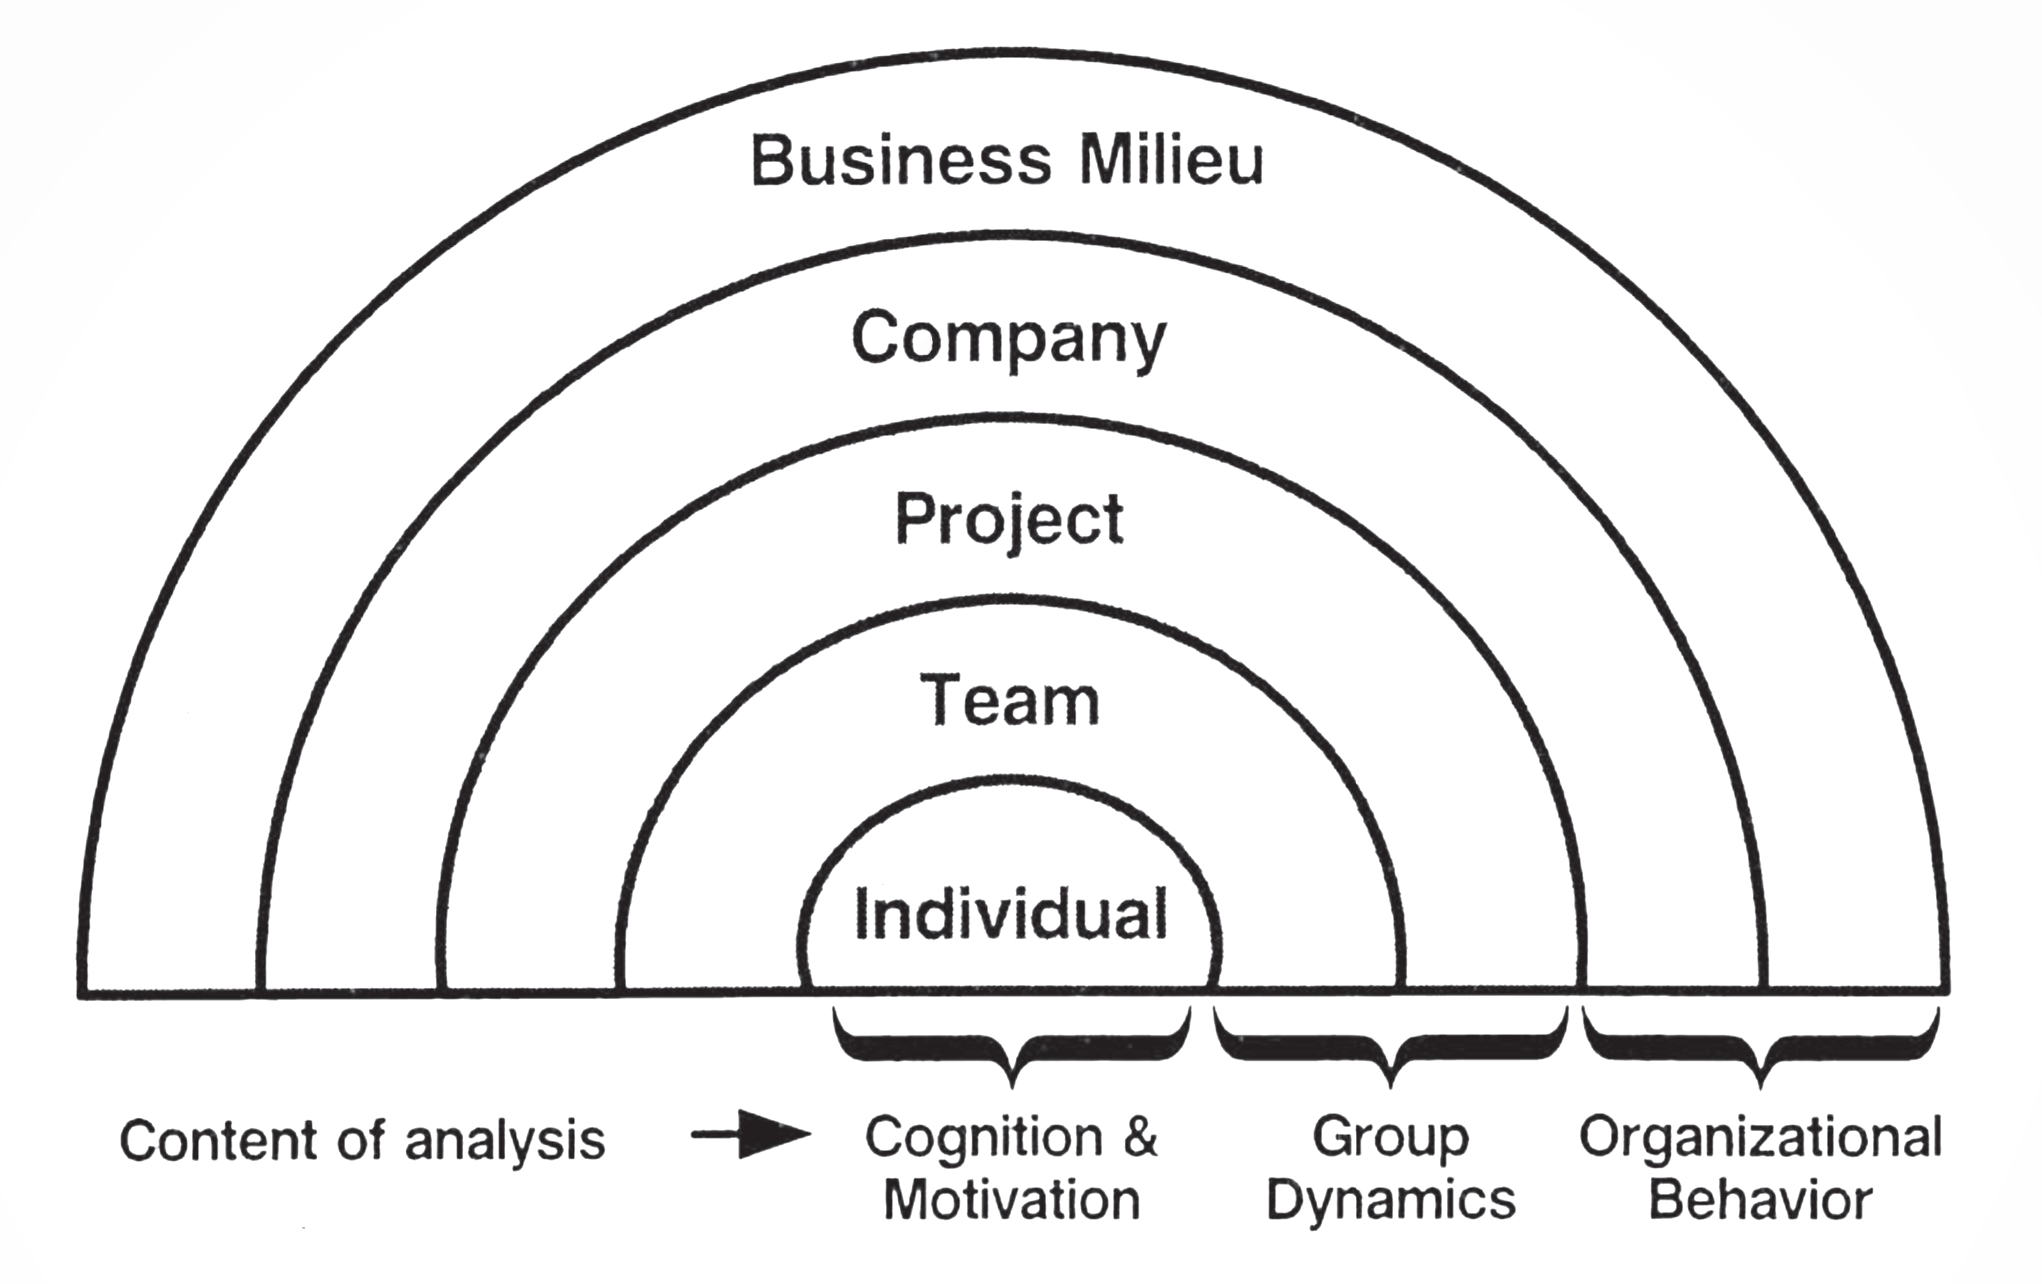
\includegraphics[width=0.7\textwidth]{layered-behavioural-model}
\caption{Layered Behavioral Model of Software Development}
\label{fig:layered-behavioural-model}
\end{figure}
They stated that ``the layered behavioral model focuses on the behavior of the humans creating the artifact, rather than on the evolutionary behavior of the artifact through its developmental stages'' \autocite[254]{curtis_psychology_1990}.
Confirming Curtis' findings, Gerald M. Weinberg already presented empirical studies about ``Programming as a Social Activity'' in 1971 \autocite{weinberg_psychology_1971}.
His studies also focus on the much understated social aspects of programming while most of the focus is put on tools for helping the individual developer, and forgetting about group, team and project communication.

Regarding communication, \textcite{curtis_psychology_1990} introduce the concept of a \emph{boundary spanner}.
During their empirical studies about the social aspects of psychology of programming they identified: ``Boundary spanners translated information from a form used by one team into a form that could be used by other teams'' \autocite[264]{curtis_psychology_1990}.
They become ``hubs for information'' \autocite[264]{curtis_psychology_1990} introducing the problem of implicit hidden knowledge that is not documented.
Regarding the title of this thesis, boundary spanners ``align mental models and models used in software development'', they transmit and translate knowledge.
The goal is not to replace boundary spanners, but merely inviting more and more people in the software development process to take part in transferring knowledge, spanning boundaries and talking about the same things.


\section{Statecharts}
\label{sec:statecharts}
Invented in 1983 by David Harel, statecharts are ``visual formalism for complex systems'' \autocite{harel_statecharts:_1987}.
While working on avionic systems for the Israeli Air Force, David Harel was asked to help taming the complexity of reactive systems.
A reactive system is dominated by its ``[...] reactivity; its event-driven, control-driven, event-response nature, often including strict time constraints, and often exhibiting a great deal of parallelism. A typical reactive system is not particularly data intensive or calculation intensive'' \autocite{harel_statecharts_2007}.
Reading this pretty narrow technical definition of a reactive system one might question the relevance of statecharts in everyday software.
Ian Horrocks provides an answer to this question by specifying the \emph{event-action paradigm} \autocite{horrocks_constructing_1999}.
User Interfaces are event-driven, they present screens with data and wait for user interactions.
Based on these they react, thus fulfilling all the requirements for a reactive system.
And because every software that is interacted with has some kind of user interface, all these programs can utilize statecharts as a way of handling state.

Describing a visual notation with words is contradictory, so let's take a look at \cref{fig:statecharts-example} taken out of the original paper introducing statecharts \autocite{harel_statecharts:_1987}.
This statechart describes part of the behavior of a digital wristwatch.
The rounded rectangles describe states the system can be in and the labeled arrows between these describe the state transitions.
Basically a statechart is an enhanced mixture between state diagrams and flow charts.
This also explains where the name comes from, according to David Harel the term \emph{statecharts} was the only unused combination of ``'state' or 'flow' with 'chart' and 'diagram''' in 1983.

\begin{figure}[h]
\centering
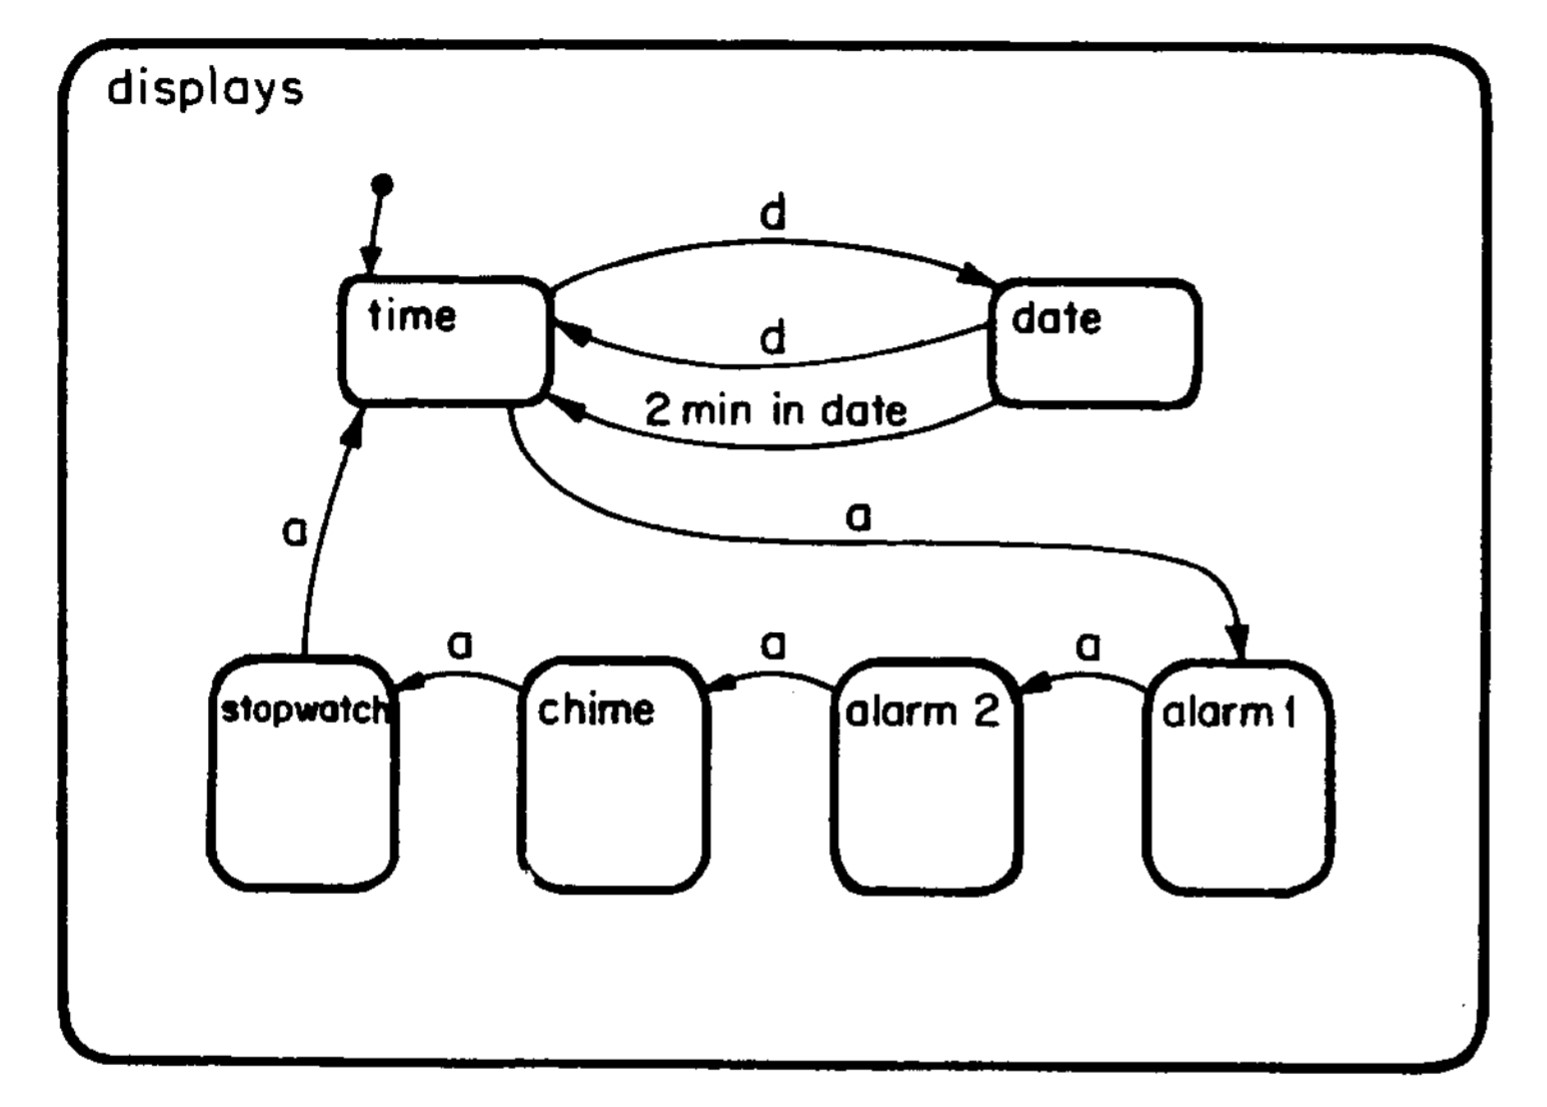
\includegraphics[width=0.8\textwidth]{small-statechart-example}
\caption{Example Statechart of a Digital Wristwatch Interface}
\label{fig:statecharts-example}
\end{figure}

As T.G.R. Green defines in \textcite[3]{green_pictures_1982} ``A \emph{program} is a succinct description of a temporal process.''
Martin Glinz describes why statecharts perfectly fit Green's definition of a program: ``Naturally, statechart models will concentrate on requirements concerning dynamic system behavior and interaction'' \autocite[1]{glinz_statecharts_2002}.
Taking a look at \cref{fig:statecharts-example} this statechart transmits this information in the following way:
\begin{itemize}
    \item The outermost box \emph{displays} is a compound state containing multiple sub-states such as \emph{time}, \emph{data}, \emph{alarm 1} and so on. In statecharts a compound state is defined by having multiple sub-states with exactly one being active at a certain point in time.
    \item The arrow originating in a black dot leading into \emph{time} specifies that this state is the initial active state of \emph{displays}.
    \item The labels \emph{d} and \emph{a} name events that can happen in a the system. In this particular example by David Harel the digital wrist watch contains four buttons, that upon pressing raise the events \emph{a}, \emph{b}, \emph{c} and \emph{d}.
    \item The arrows labeled \emph{d} between \emph{time} and \emph{date} can be translated to a toggle functionality between the time and display states of the watch.
    \item The arrow labeled with \emph{2 min in date} follows exactly its description. If the state \emph{date} has been active for two minutes and no event occurred the state \emph{time} is automatically entered.
    \item If the system is in state \emph{time} and the event \emph{a} occurs it will transition to \emph{alarm 1}, on another press of \emph{a} into state \emph{alarm 2} and so on.
\end{itemize}

One of the most important properties of statecharts in comparison to textual source code is the obviousness of valid and invalid transitions.
Users of the statechart can immediately conclude which events are possible in which state.
Another property of statecharts is that events not allowed in the currently active state are simply ignored instead of causing errors, thus leading to more robust and less faulty programs \autocite{horrocks_constructing_1999}.
For a full overview of the available features of statecharts please refer to \textcite{harel_statecharts:_1987}.

\subsection{The Goals Behind}
\label{sub:goals-behind-statecharts}
In \citeyear{harel_statecharts_2007}, David Harel published his personal story behind statecharts titled ``Statecharts in the Making: A Personal Account'' \autocite{harel_statecharts_2007}.
In this paper he talks about his psychological ideas and observations during the development of statecharts in the eighties.
Apart from creating a \emph{visual formalism} for reactive systems, he wanted to create a notation for \emph{model-based development} (which became really popular with the Unified Modeling Language [\textcite{cook_unified_2017}]) and an executable model where the behavior ``can and should be executed just like [with] conventional computer programs [...]'' \autocite[1]{harel_statecharts_2007}.
This technical goals lay the foundation for two of his greater goals that can be attributed to social psychology \autocite[3--4]{harel_statecharts_2007}:
\begin{itemize}
    \item ``The goal was to try to find, or to invent for these experts, a means for simply saying what they seemed to have had in their minds anyway.''
    \item ``The goal was to find a way to help take the information that was present collectively in their heads and put it on paper, so to speak, in a fashion that was both well organized and accurate.''
\end{itemize}

The above mentioned \emph{executability} is another fundamental idea of statecharts \autocite[7]{harel_modeling_1998}, because of the simulation aspect taking a lot of cognitive load off the developer.
Back in the eighties executable models weren't the standard, because the graphics and input capabilities of computers were not comparable to the ones used today, but even then David Harel imagined ``[...] graphical workstations with large (blackboard size?) displays of fantastic resolution [...]'' \autocite[272]{harel_statecharts:_1987}.
More than 30 years later, devices like the Microsoft Surface Hub\footnote{\url{https://www.microsoft.com/en-us/surface/business/surface-hub-2}} exist that perfectly match this description.
Combined with Bret Victor's ideas of instant code executability \autocite{victor_inventing_2012} this could be the perfect match for an interactive development environment based on statecharts.

\subsection{Aligning Thoughts with Fractal Architectures}
\label{sub:aligning-thoughts-with-fractal-architectures}
Comparing different approaches to user interface development, André Staltz coined the term \emph{fractal architecture} as ``[an] architecture is said to be fractal if subcomponents are structured in the same way as the whole is'' \autocite{staltz_unidirectional_2015}.
Fractals are a mathematical concept of geometric figures that appear the same at different levels.

As described earlier, statecharts feature the concept of compound states, wherein states can be nested inside each other.
This property perfectly maps to ``geometric figures that appear the same at different levels'' and André Staltz's definition of fractal architectures.
This state nesting allows to refine the behavior of a certain state by adding sub-states and thus adapting to new requirements without breaking others \autocite{harel_statecharts:_1987}.
\textcite{leveson_experiences_1991} discuss the two main strategies of transforming requirements into software: \emph{top-down} and \emph{bottom-up}.
The top-down strategy is based on top-down refinement where requirements are deconstructed one by one, starting from the most abstract one transitioning down the tree of requirements.
Unfortunately, this process only works for experts possessing a huge knowledge in software design and the problem domain.
The bottom-up strategy, on the other hand, is characterized by less upfront thoughts about design and immediately starting with the implementation of requirements at a very detailed level.
A major problem using this approach is that a well designed software architecture is nearly impossible to reach, especially as applications get larger \autocite{horrocks_constructing_1999}.
As stated in \textcite{leveson_experiences_1991}, programmers constantly switch between those two strategies while developing software.

This is exactly the point where the fractal nature of statecharts can be aligned with the characteristics of programming.
States itself can be nested (\emph{bottom-up}) as well as refined using sub-states (\emph{top-down}), directly resembling the composition and decomposition of requirements as shown by \textcite{leveson_experiences_1991}.
\textcite{glinz_statecharts_2002} already started research in the direction of transforming requirements into statecharts, but only from a technical and not from a psychological perspective.


\section{Hole-Driven Development}
\label{sec:hole-driven-development}
The term \emph{Hole-Driven Development} is not yet scientifically defined, but based on other programming concepts like \emph{Type-Driven Development} \autocite{brady_type-driven_2017} or \emph{Test-Driven Development} \autocite{mccracken_digital_1957}.
The main idea stems from the \emph{Agda} programming language\footnote{\url{https://wiki.portal.chalmers.se/agda/pmwiki.php}} where \emph{holes} are called \emph{goals}.
Apart from Agda, other languages such as Haskell\footnote{\url{https://www.haskell.org/}} and Idris\footnote{\url{https://www.idris-lang.org/}} feature the concept of holes.
The common properties of those languages is their functional nature and a very sophisticated type system.
These two aspects lay the foundation for Hole-Driven Development as currently understood.

Simply said, a \emph{hole} declares a missing part in an application.
\textcite{gamari_haskell_2019} contains the up to now most comprehensive description of the concept of holes, while \textcite{brady_type-driven_2017} created the example shown in the following section.

\subsection{Example in Idris}
\label{sub:hole-driven-development-in-idris}
The Idris program in \cref{fig:idris-program-hole} demonstrates the simplest possible hole.
In Line \verb|2| the function \verb|main| is defined that should print something (using the standard library function \verb|putStrLn|) to the console.
The ``hole'' part of this program is \verb|?greeting|.
Signaling a hole, the question mark tells the Idris compiler that something in this program is missing that the developer didn't specify yet.
The syntax using a question mark resembles a question to the compiler.

\begin{figure}[h!]
\begin{lstlisting}[language=Haskell,firstnumber=1]
main : IO ()
main = putStrLn ?greeting
\end{lstlisting}
\caption{Hole-Driven Development in Idris}
\label{fig:idris-program-hole}
\end{figure}

Edwin Brady coined the phrase ``the compiler as your lab assistant'' \autocite{brady_type-driven_2017}.
His imagination of a compiler is one of a counterpart one interacts or pair-programs with.
One tells the compiler all the things that are currently in ones mind and as a reward one can ask questions and the compiler will try to answer those based on the knowledge already provided.
In terms of psychology, this is a pretty human way of interacting with the computer.

A practical example of this ideas looks like the following output of Idris' interactive command line interface.
Using \verb|:t greeting| one can ask the compiler for the type of the hole ``greeting''.
As an answer one gets \verb|greeting : String| which signals that the missing value is of type String, or in a non-technical terminus simply a text to complete the program definition.

\begin{verbatim}
*Hello> :t greeting
--------------------------------------
greeting : String
\end{verbatim}

In contrast to the previous example, if you just try to use \verb|greeting|, the Idris compiler tells you that you have a hole in your program labeled \emph{greeting} of type String.
This shows the communication process Edwin Brady talks about.

\begin{verbatim}
*Hello> greeting
?greeting : String
\end{verbatim}

``Holes allow you to develop programs \emph{incrementally}, writing the parts you know and asking the machine to help you [...]'' \autocite[21]{brady_type-driven_2017}.
Stepping a little bit back and comparing this way of developing software to how software development processes evolved (see \cref{sub:traditional-vs-agile}), the similarities are unmistakable.
Let's take a look at how holes are simulated in programming languages that don't support this feature natively before we get to psychological observations that were already discovered in the field of psychology of programming.

\subsection{Simulating Holes}
In languages that do not provide the feature of typed holes, programmers tend to come up with alternative solutions to holes without knowing of their existence.
Psychological research (see \cref{sub:incomplete-thoughts}) indicates that the process of creating these holes is so natural to the thought process that even within languages without the concept of holes, developers find a way of expressing those.
There are mainly two ways of simulating holes:
\begin{enumerate}
\item One might throw exceptions such as \verb|NotImplementedException|, as documented in \textcite{microsoft_notimplementedexception_2020}, to signal that a feature is not yet implemented.
\item Comments are another common way of deferring development of a particular method or feature, marking the comment as a ``hole'' prefixing it with \verb|TODO:|. E.\,g. in C\#\footnote{\url{https://docs.microsoft.com/en-us/dotnet/csharp/}} this looks like \verb|// TODO: Load state from previously suspended application|. Interactive development environments are able to parse this information and provide an overview of to-dos as shown in \textcite{hogensen_use_2019}.
\end{enumerate}
These two concepts might look like sufficient surrogates at first, so what are the differences to real holes?
\begin{itemize}
    \item The previously described interaction with the compiler is missing completely.
    \item By using exceptions the program crashes at run-time, which results in buggy software. Additionally, there is no real overview of all the simulated holes. One has to do a text-based search for the exception name.
    \item Utilizing comments doesn't result in the program crashing, rather not adhering to the specifications without any note at run-time. This might lead to incorrectly behaving software.
    \item Both approaches act like a ``do-it-later'' approach, without actively reminding the developer at a later time.
\end{itemize}

\subsection{Incomplete Thoughts}
\label{sub:incomplete-thoughts}
In the meta-analysis \citetitle{visser_expert_1990} \citeauthor{visser_expert_1990} conducted in \citeyear{visser_expert_1990} collected thinking processes and strategies of expert programmers \autocite{visser_expert_1990}.
Comparing breadth-first and depth-first design methodologies, they found out that expert developers vary in their usage and most of the time combine both strategies.
One commonality was the observation that the developers under research were observed making ``notes to themselves'' \autocite[241]{visser_expert_1990}.
Experts usually excel at maintaining relevant information in memory, nevertheless this memory capacity is limited and working on one problem might relate to other problems until there is not enough capacity left and they start taking those notes.
They conclude that ``[...] before introducing the constraints of actual programming languages, experts very often use[d] a personal pseudo-code'' \autocite[242]{visser_expert_1990}.

Combining this research, it seems plausible that real holes enhanced with comments could lead to a programming language that lets developers specify the already thought-out ideas in executable source code while still letting them express their ideas in written natural language with the advantage of the programming environment caring about their ideas.


% The internal model is iteratively finetuned during requirements specification development to mimic our understanding of the process with sufficient detail to achieve the desired control performance.
\chapter{Psychological Foundation (14)}

\section{Psychology of Programming (4)}
- "The origins of PoP date back to late 1970s and early 1980s, when researchers realized that programming tools and technologies should not be evaluated based on their computational power only, but also on their usability from the human point of view, that is, based on their cognitive effects." \autocite[4]{sajaniemi_psychology_2008}
- "Disappointingly little theory and few research paradigms from these fields have been imported into the psychological study of programming." \autocite[253]{curtis_psychology_1990}
- Motivation of Computer Scientists vs. Psychologists \autocite[4]{sajaniemi_psychology_2008}
- 2READ: \autocite{detienne_expert_1990}
- Assistance to the design activity \autocite[246--247]{visser_expert_1990}
- 2READ: \autocite{watt_syntonicity_1998}
- \autocite{weinberg_psychology_1971}
\subsection{Programming as Theory Building}
- \autocite{naur_programming_1985}
- \url{https://catenary.wordpress.com/2011/04/19/naurs-programming-as-theory-building/}
- \url{https://twitter.com/ruthmalan/status/1245058319435300866}
- \url{https://twitter.com/ruthmalan/status/1144563675128303616}
\subsection{Metaphors}
- \autocite[239--240]{naur_programming_1985}
- METAPHORS WE COMPUTE BY - Alvaro Videla
  - \url{https://alvaro-videla.com/2017/01/metaphors-we-code-by.html}
  - \url{https://hooktube.com/watch?v=hKOzJWNRBWA&feature=youtu.be}
  - "Sometimes our tools do what we tell them to do. Other times, we adapt ourselves to our tools’ requirements" - Nicholas Carr

\section{Visual Notations}
- Introduction + "picture superiority effect" \autocite[756]{moody_physics_2009}
- "Visual notations are uniquely human-oriented representations: Their sole purpose is to facilitate human communication and problem solving" \autocite[757]{moody_physics_2009}
- Why Visual Representation Is Important \autocite[758--759]{moody_physics_2009}
- "Spatial Fashion in Smalltalk" [Bret Victor - The Future of Programming](https://hooktube.com/watch?v=8pTEmbeENF4) (19:34)
- [Image: The Danger of Visual Representation](https://twitter.com/parport0/status/1253716518363369475?s=21)
- [Visual Representation - The Encyclopedia of Human-Computer Interaction, 2nd Ed.](https://www.interaction-design.org/literature/book/the-encyclopedia-of-human-computer-interaction-2nd-ed/visual-representation)
\subsection{Dual Coding Theory}
- "In a position in-between we can cite Agnyal [1], who claims that using two synchronised notations (graphical-textual) for the domain model improves its maintainability." \autocite[3]{melia_comparison_2016}
- In regards to Statecharts and modifications \autocite[38--39]{leveson_experiences_1991}
- \url{https://en.wikipedia.org/wiki/Dual-coding_theory}
\subsection{Visual Programming (3)}
- "information exposure" \autocite[34]{leveson_experiences_1991}
- Readability and Reviewability \autocite[37-38]{leveson_experiences_1991}
- Some Notes on Visual Programs \autocite[5--6]{green_pictures_1982}
- Flowcharts $\rightarrow$ Statecharts (\ref{sec:statecharts}) \autocite[8]{green_pictures_1982}
- "backwards tracing is easier in graphical notation than in programming languages." \autocite[20]{green_pictures_1982}
\subsection{History}
\subsection{Problems}
- \autocite{melia_comparison_2016} Only examined research on one specific notation.
    - "Petre [36] points at the fact that, since using textual modelling languages is similar to programming, the learning curve is lower than for graphical representations" \autocite[3]{melia_comparison_2016}
    - "Subjects in the experiment performed significantly better both for analysability coverage and modifiability efficiency with a textual notation" \autocite[26]{melia_comparison_2016}
    - "The most relevant threat to the validity of our results is that the quasi-experiment was performed with students and small models" \autocite[26]{melia_comparison_2016}
    - Junior Developers, Trained using Textual Notation
- on putting things in boxes (subroutines) \autocite[23]{green_pictures_1982}
- 2READ: \autocite{bresciani_pitfalls_2015}
- \autocite{cook_unified_2017}

\section{Solving Complex Problems (3)}
- Complexity \autocite[5--11]{ousterhout_philosophy_2018}
- "Ill-defined problems" \autocite[236]{visser_expert_1990}
- Programming Languages: Different Levels of analysis and flow of development (\ref{sec:hole-driven}) \autocite[242--244]{visser_expert_1990}
\subsection{In Groups}

\section{Mental Models (5)}
- Cognitive Models (\ref{sec:applications}) \autocite[276]{kitchenham_research_1990}
- Cognitive Issues in Software Development regarding Design Notations (Thinking in States, Mathematical vs. Structured Methods) \autocite[281--282]{kitchenham_research_1990}
- 2READ: \autocite{gentner_mental_2014}
- 2READ: \autocite{dutke_mentale_1994}
- 2READ: \autocite{herczeg_software-ergonomie_2018}
- 2READ: \autocite{wandmacher_software-ergonomie_1993}
\subsection{Sharing Mental Models}
- Transferring Mental Models "The specification must be formal enough for us to use as a basis for a safety analysis. It must also be readable enough for noncomputer experts to read and review and be usable for both building and certifying TCAS I1 systems." \autocite[32]{leveson_experiences_1991}

- Communicating Mental Models \autocite[275]{kitchenham_research_1990}
- Sharing Designs \ref{sec:literate-programming} \autocite[282]{kitchenham_research_1990}
- Transferring Knowledge \autocite[234--235]{naur_programming_1985}
\subsection{Cross-Domain}
- Mental Models in Statecharts \autocite[2]{harel_statecharts_2007}
\subsection{Human-Computer vs. Human-Human Interaction (Literate Programming)}
- \url{https://en.wikipedia.org/wiki/Literate_programming}

\section{Working Memory}
\label{sec:working-memory}

\section{Social Aspects of Team Communication (2)}
\chapter{Implications}
\todo{that's new}
\label{chap:possible-applications}
\epigraph{``More effective tools could be built if we understood the creation process and knew what tools were needed to support human weaknesses and magnify human strengths.''}{\textit{Barbara Kitchenham}}
\noindent
This quote by Barbara Kitchenham applies to tools in general.
Speaking of tools used in software development \textcite{kitchenham_research_1990} further specify these as ``thinking tools for thinking.''
In this chapter the various ideas and findings are presented that build upon the foundation presented in \cref{chap:technological-foundation} and \cref{chap:psychological-foundation}.

As shown in \cref{sec:characteristics-of-software-development-processes} software development processes involve a lot of participants.
The customer or user imagines the perfect product, the requirements engineer thinks in user stories, testers use acceptance criteria and developers think in source code.
Each of them creates an own mental model trying to solve one part of the common problem.
Approaching a common problem with different mental representations results in the use of different tools, thus speaking ``different languages'' requiring translations or cross-domain knowledge and understanding of the people involved.

The title of this thesis promises the alignment of mental models to models used in software development.
Considering specific mental models or models used in software development and creating counterparts would solve those problems in specific cases.
Of much greater impact would be the creation of a software modeling tool that is aligned to the nature of mental models, thus enabling modeling in software development in such a way that it is analogous to developing mental models.


\section{Combining Statecharts and Hole-Driven Development}
\label{sec:combining-statecharts-and-hole-driven-development}
To the knowledge of the author, statecharts and hole-driven-development have not yet been combined.
By integrating the concept of holes into the notation of statecharts, the visual formalism as introduced by \textcite{harel_statecharts:_1987} is extended by the property of \emph{incompleteness}.
\cref{fig:statecharts-hole-example} exemplifies how such an extension may look like.
The goal of this thesis is not to invent a notation for such an extension.
Merely the author explains ways of how such a combination could improve the process of software development backed by psychological research.
\begin{figure}[h]
\centering
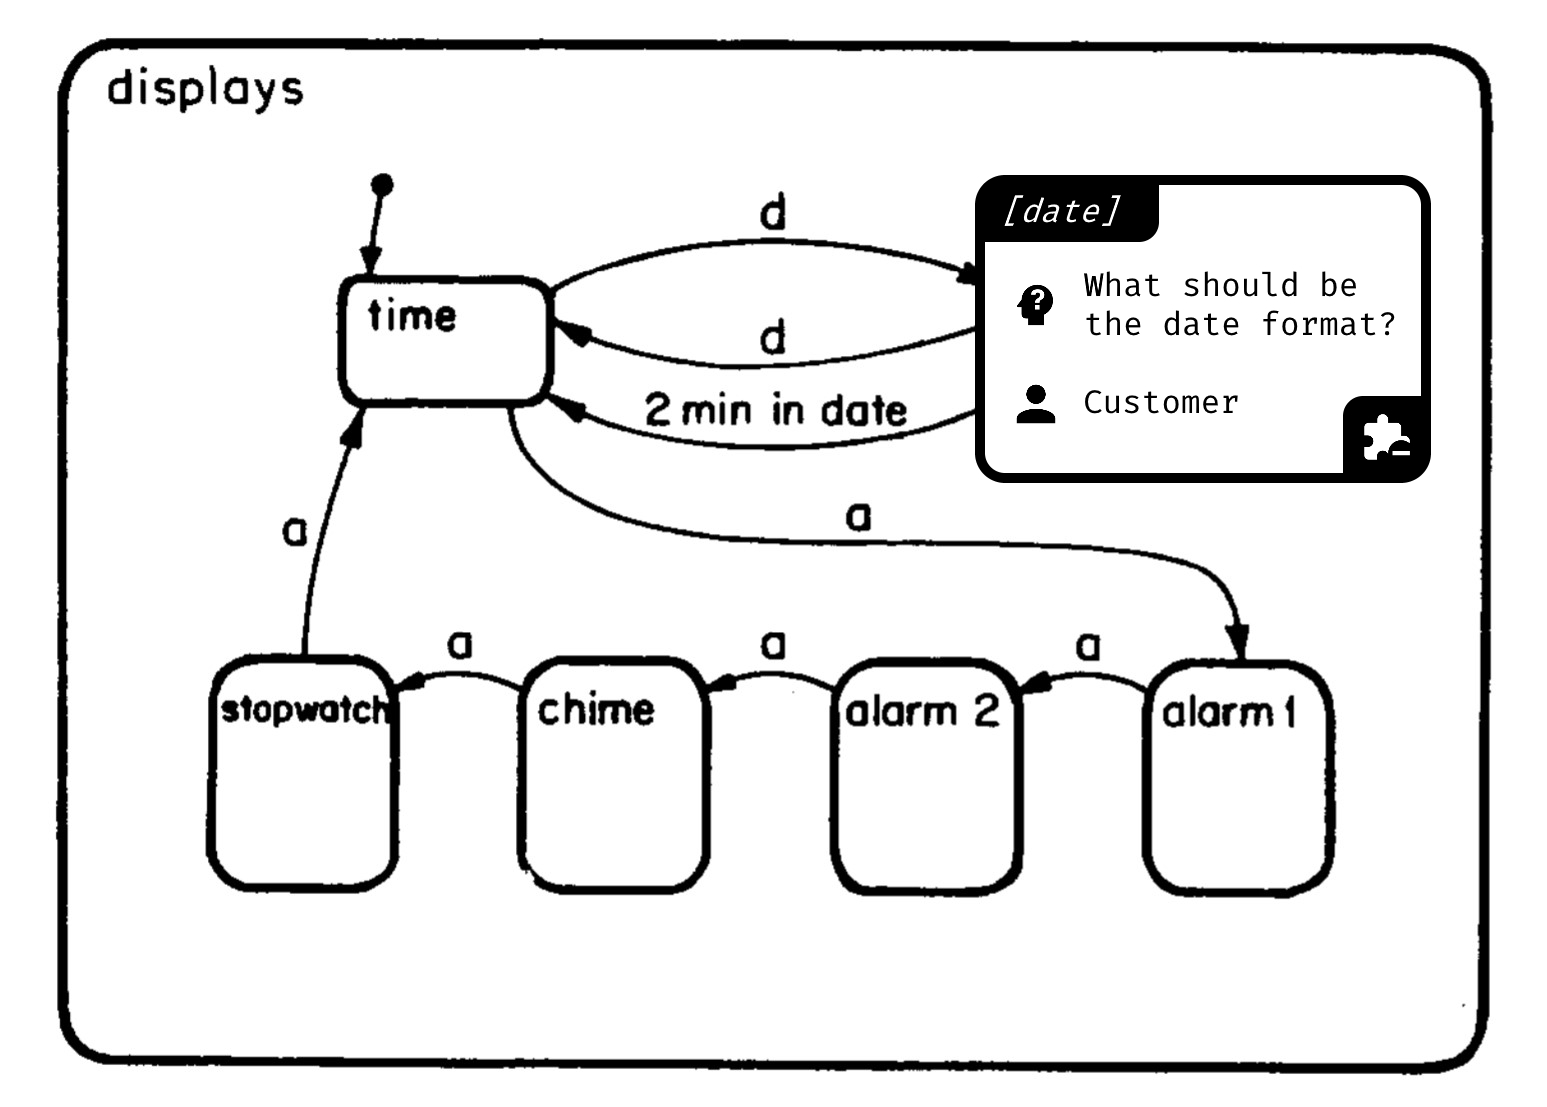
\includegraphics[width=0.8\textwidth]{images/statechart-hole-example}
\caption{Statechart including the state hole ``date''}
\label{fig:statecharts-hole-example}
\end{figure}
In comparison to \cref{fig:statecharts-example}, the state \emph{date} is now replaced by a \emph{state hole} named date, which is indicated by the icon of a missing puzzle piece as well as the name put in brackets.
As explained in \cref{sub:hole-driven-development-in-idris} typed holes are labels that serve as questions to the compiler.
Not targeted at compilers, but at other participants in the software development process, holes in statecharts convey way more information.
A hole without any context is useless, thus the most important information is the reason for the creation of a hole.
In this example, somebody in the software development process (probably a developer or requirements analyst) was unsure about the date format that should be used while presenting the date on the watch.
Intended as a tool simplifying communication, the role of a person intended to respond (customer in this example) is specified as well.
Summarizing this description the creator of this hole might have thought: ``I already know there should be a state called date in the behavior of the watch, but I am unsure about the date format to display, thus I am asking the customer (or a product manager acting as the customer) for clarification.''

By combining statecharts and hole-driven development it seems possible to
\begin{itemize}
    \item \emph{specify requirements} using a visual formalism \autocite{leveson_experiences_1991},
    \item create a \emph{shared model of understanding} (see \cref{sec:mental-models}),
    \item that can be directly \emph{executed} \autocite{harel_statecharts:_1987},
    \item and is \emph{aligned to the thought process} of developing software (see \cref{sub:aligning-thoughts-with-fractal-architectures}, \cref{sec:psychology-of-programming}),
    \item while \emph{improving communication} in the software development process (see \cref{sub:insights-from-psychology}).
\end{itemize}
Based on their conducted research, \textcite{visser_expert_1990} identified five rules for tools that assist the design activity.
Does the combination of statecharts and hole-driven development adhere to these rules?


% statecharts are just a static representation of data -> declarative programming
% during this chapter properties of mental models
% - based on beliefs, generate descriptions
% - anticipate behavior
% - might be erroneous and incomplete
% - flexible
% - temporary
% - adapt to new information
% - capability of simulation

\subsubsection{1\textsuperscript{st} rule: assisting the management of working memory}
The cognitive system \emph{working memory} acts as a buffer between the sensory register and the long-term store, its capacity is limited and information is only held temporarily \autocite{herczeg_software-ergonomie_2018}.
Regarding the performance of the working memory, $7 \pm 2$ chunks can be stored for around $15-30$ seconds \autocite{herczeg_software-ergonomie_2018}.
As presented by \textcite{victor_inventing_2012} these limitations seriously restrict the understanding and mental simulation of a program's behavior, thus longing for interactive visual alternatives.
Based on the results of various studies \textcite{dutke_mentale_1994} states that on principle visualizations support cognitive processes, while entailing the major risk of a mental overload.
Such an example is presented in \cref{fig:full-wristwatch-statechart} \autocite{harel_statecharts:_1987}.
\begin{figure}[h]
\centering
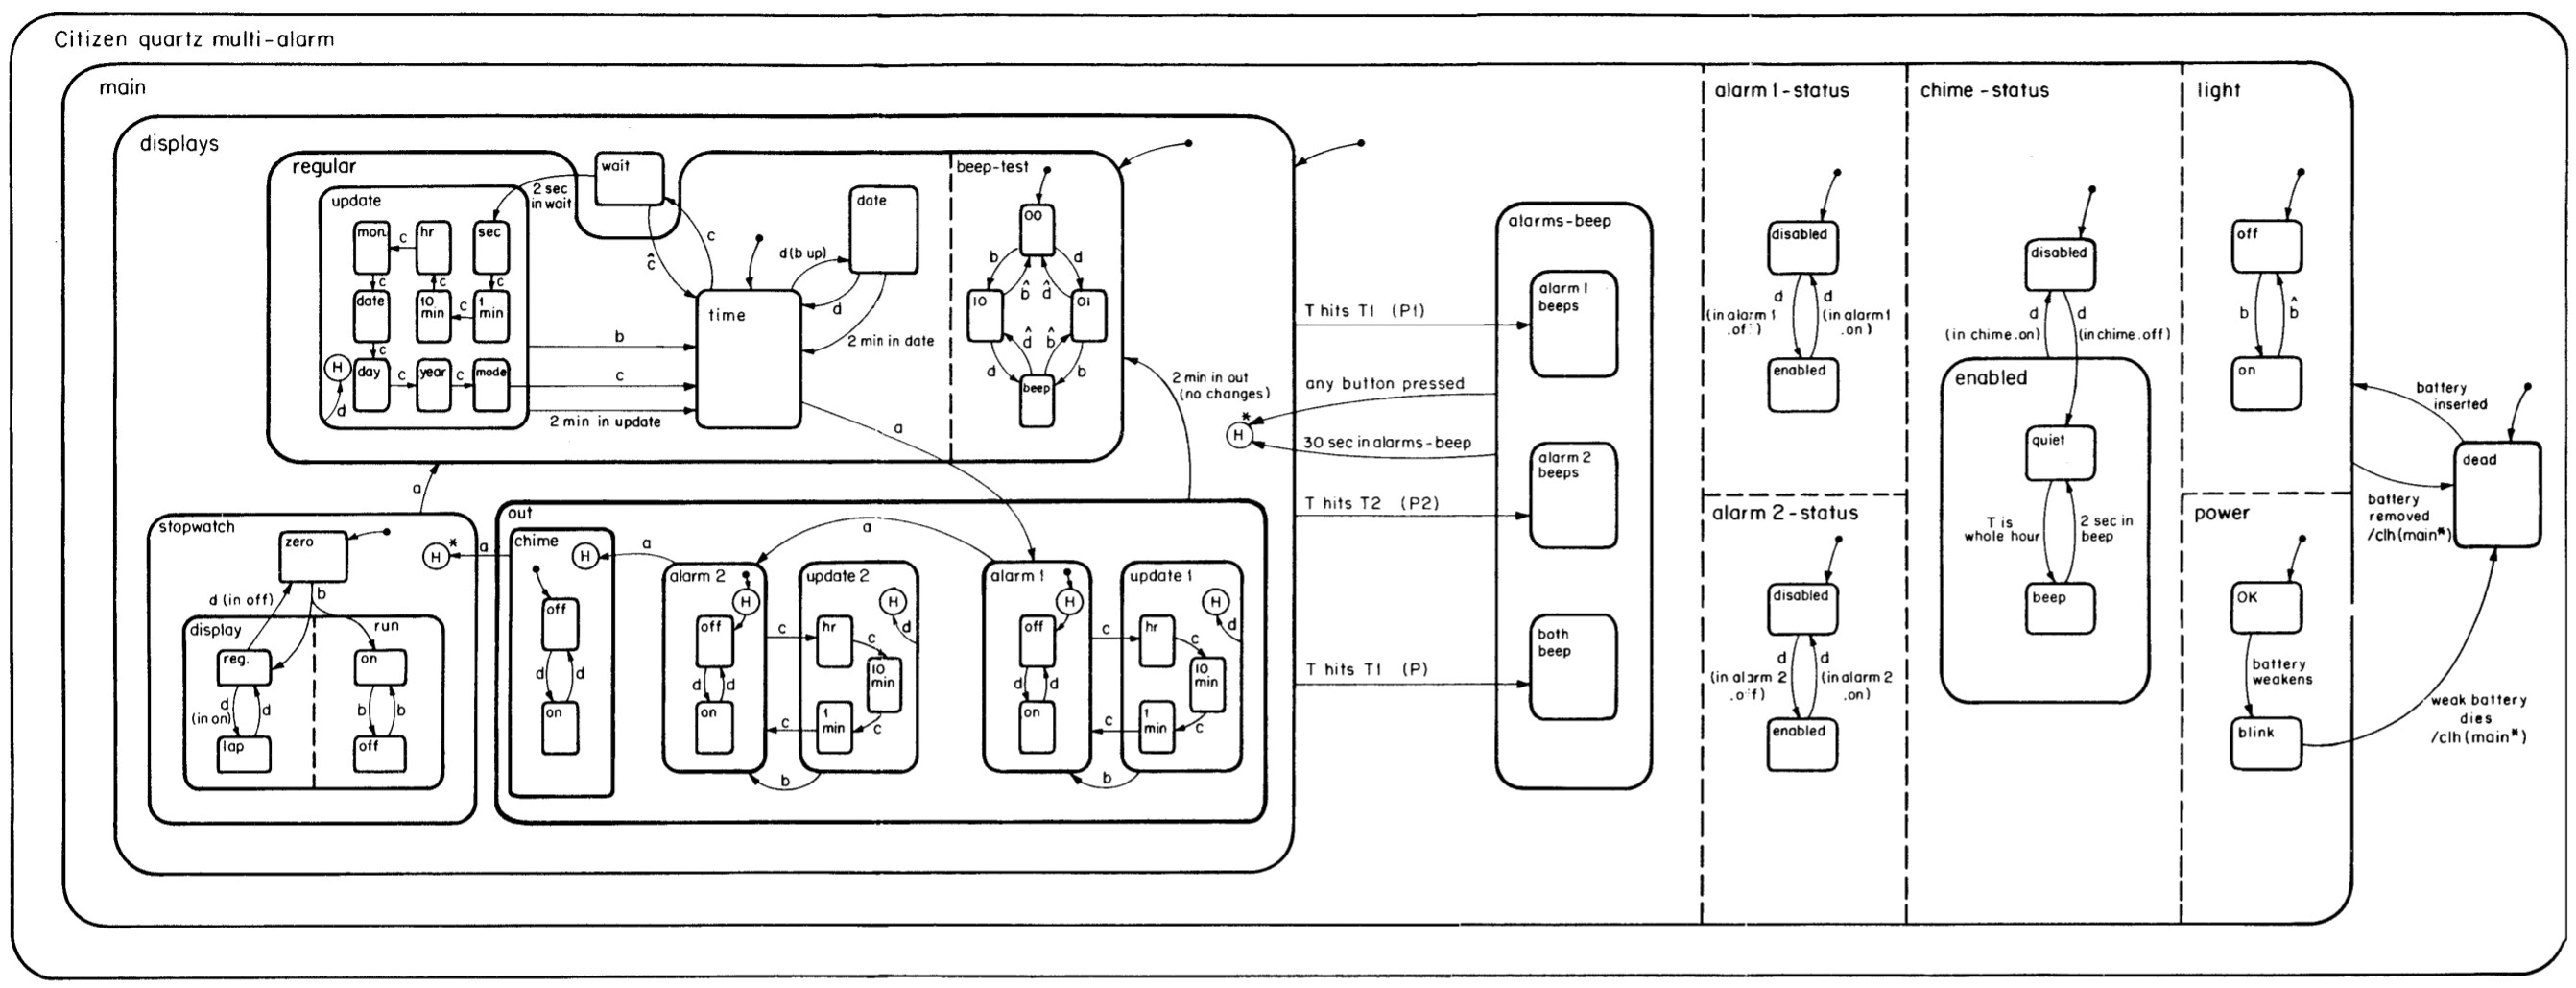
\includegraphics[width=\textwidth]{images/full-watch-statechart}
\caption{Full Statechart of a Digital Wristwatch Interface}
\label{fig:full-wristwatch-statechart}
\end{figure}
Despite the fact that the behavior of the full system is visible at one glance, this statechart is impractical to use in this form \autocite{harel_statecharts:_1987}.
It lost a model's character of abstraction.
For getting an overview of the full system it is not abstract enough and for understanding a certain part of the wristwatch there is too much noise \autocite{dutke_mentale_1994}.

Due to the fractal nature of statecharts (see \cref{sub:aligning-thoughts-with-fractal-architectures}) the various sub-states can be folded away and the same model can be visualized as \cref{fig:simplified-wristwatch-statechart}.
It is important to note that the underlying model did not change, only its representation.
\begin{figure}[h]
\centering
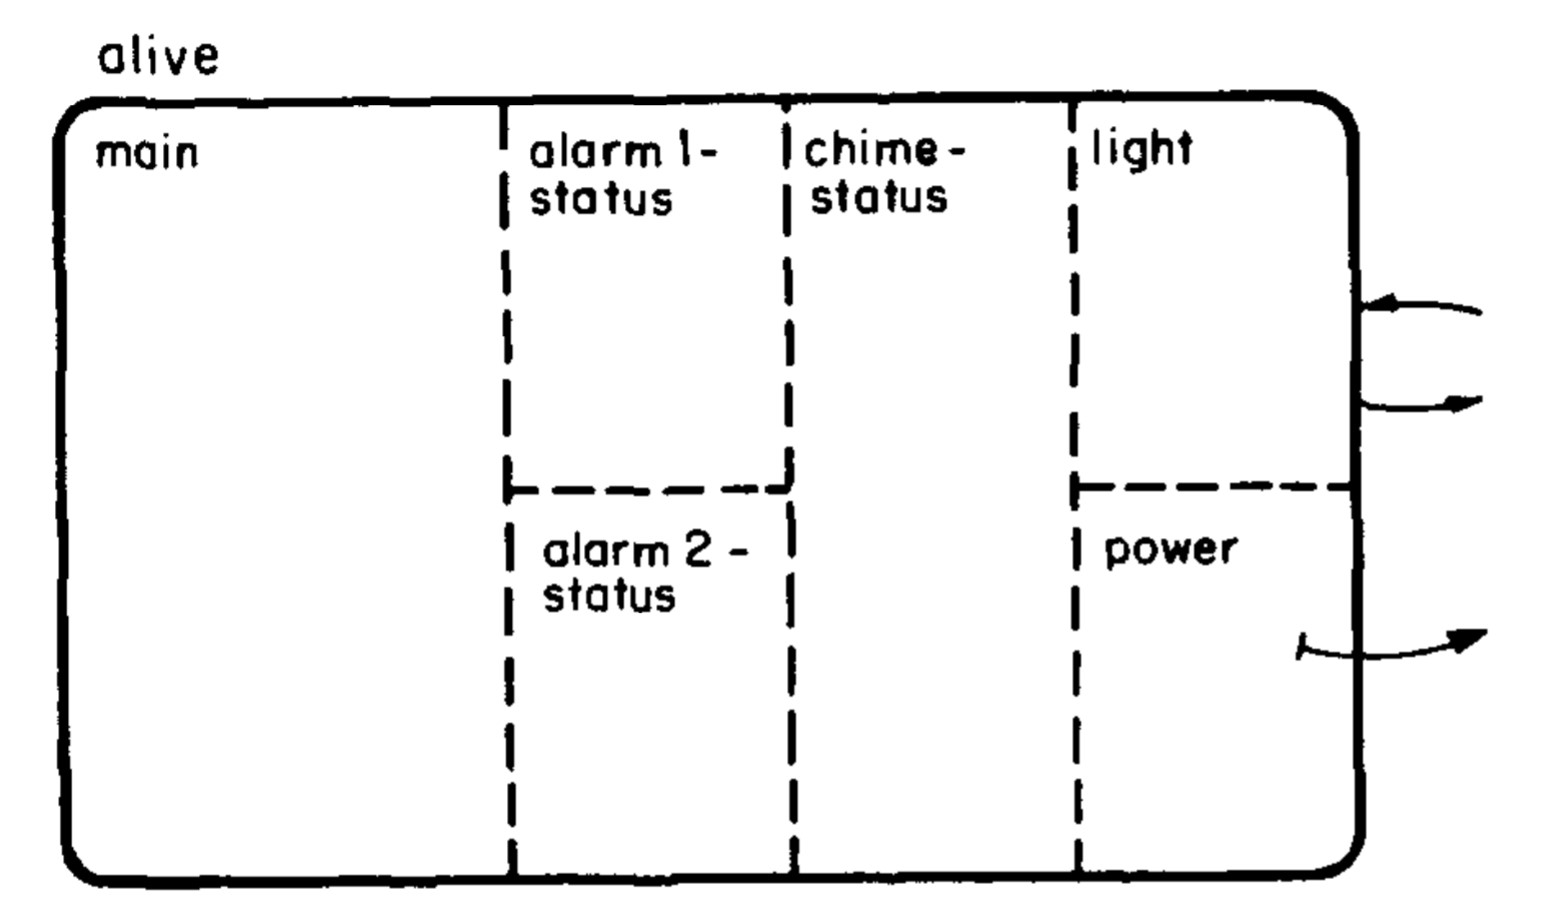
\includegraphics[width=0.8\textwidth]{images/abstract-watch-statechart}
\caption{Simplified Statechart of a digital Wristwatch}
\label{fig:simplified-wristwatch-statechart}
\end{figure}
As the limitations caused by technology described in \textcite{harel_statecharts:_1987} were overcome, tools like the XState Visualizer\footnote{\url{https://xstate.js.org/viz/}} emerged, allowing developers to fold and unfold states at any time.
This interactive way of creating different abstractions of the same model allows the selective use of working memory.

\subsubsection{2\textsuperscript{nd} rule: enabling the use of libraries and design schemata}
As mentioned by \textcite{visser_expert_1990} reusability is a major aspect while creating tools that assist system design.
Reusing solutions of already solved problems is as important as shared knowledge about design schemata.
Again the fractal nature of statecharts enables this property as defined by \citeauthor{visser_expert_1990}.
Being able to create self-contained elements allows transferring these between projects or taking over existing solutions into the current project.
Statechart implementations such as XState\footnote{\url{https://xstate.js.org/}} or Statecharts.NET\footnote{\url{https://github.com/bemayr/Statecharts.NET/}} simply reuse the infrastructure of the programming language they are written in.

\subsubsection{3\textsuperscript{rd} rule: assisting the articulation of top-down and bottom-up components}
Regarding problem decomposition strategies \textcite{visser_expert_1990} differentiate between the top-down and bottom-up strategy.
Programmers decomposing a problem top-down start at the root node of the solution tree and descend down against more concrete solutions, never going back up.
As discovered by \textcite{brooks_towards_1977} there are only rare cases a clear top-down strategy really works.
In these cases the programmers have to be experts and possess detailed knowledge in the problem domain \autocite{dutke_mentale_1994}.
Bottom-up strategies are defined by starting with the solution to one specific problem and creating the design in the process of solving particular problems.
This approach to problem decomposition is usually taken by beginners and results in worse architecture than a well-thought-through top-down approach \autocite{visser_expert_1990}.
In reality a combination between both of those is used where stepping back up in the solution tree followed by descending down again is called ``backtracking''.

As suggested by \textcite{visser_expert_1990} programming languages should support different levels of analysis and various flows of development, as the human brain works best not being forced to comply to one specific strategy.
Already explained in \cref{sub:aligning-thoughts-with-fractal-architectures}, the fractal nature of statecharts enables programmers to nest and refine states as they create their solution tree.
This model directly maps to the top-down strategy (refining states) and the bottom-up strategy (nesting states), thus assisting system design as intended by \textcite{visser_expert_1990}.

\subsubsection{4\textsuperscript{th} rule: enabling prospective strategies}
The prospective declarative problem decomposition strategy helps at solving problems ``where the complex structure of the input files and the relationships between them introduce strong and complex constraints on the program structure'' \autocite[243]{visser_expert_1990}.
In contrast to the prospective procedural strategy where statements are written according to a mental execution strategy the problems are too complex to be guided by already available procedures.
This type of problem is called ``ill-structured'' \autocite[236]{visser_expert_1990}.

For those kinds of problems it is especially important to provide tools that enable decomposition, because initially the problem space is too large to be solved at once \autocite{dutke_mentale_1994}.
By providing the aforementioned assistance in top-down and bottom-up problem decomposition the concept of statecharts already provides help for solving complex problems.
Enabling prospective strategies is achieved by the combination with hole-driven development.
By introducing holes programmers can write themselves notes to the future that cannot be forgotten, because when trying to execute the statechart it will fail with an incomplete definition.
\cref{fig:vs-task-list} shows the \emph{Task List} of the integrated development environment Visual Studio 2019 \autocite{hogensen_use_2019}.
\begin{figure}[h]
\centering
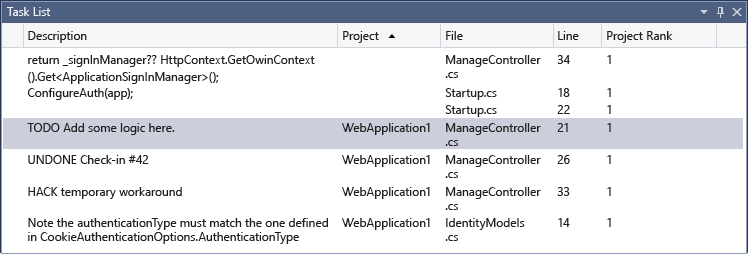
\includegraphics[width=0.9\textwidth]{images/task-list}
\caption{Task List of a modern Integrated Development Environment}
\label{fig:vs-task-list}
\end{figure}
This concept can be applied to the combination of statecharts and hole-driven development presenting an overview of all currently existing holes.
Due to the additional information provided by holes as described in \cref{chap:possible-applications} this list can be targeted for specific participants in a software project keeping the mental overload as small as possible.
Furthermore instead of showing the file location, the superstate of the hole can be displayed, enhancing the information presented with even more context.
Instead of keeping the tasks to do in mind or using external tools, developers, system analysts, architects and other people in the software development process can be guided by the task list based on the holes in the statechart in a real \emph{single} source of truth.


\subsubsection{5\textsuperscript{th} rule: assisting simulation}
As described in \cref{sec:mental-models} the simulation aspect of mental models is fundamental to their applicability.
Statecharts, being a model as well, provide this same aspect of simulation.
\cref{fig:xstate-simulation} shows this simulation aspect in practice, the used tool is called XState Visualizer\footnote{\url{https://xstate.js.org/viz/}}.
\begin{figure}[h]
\centering
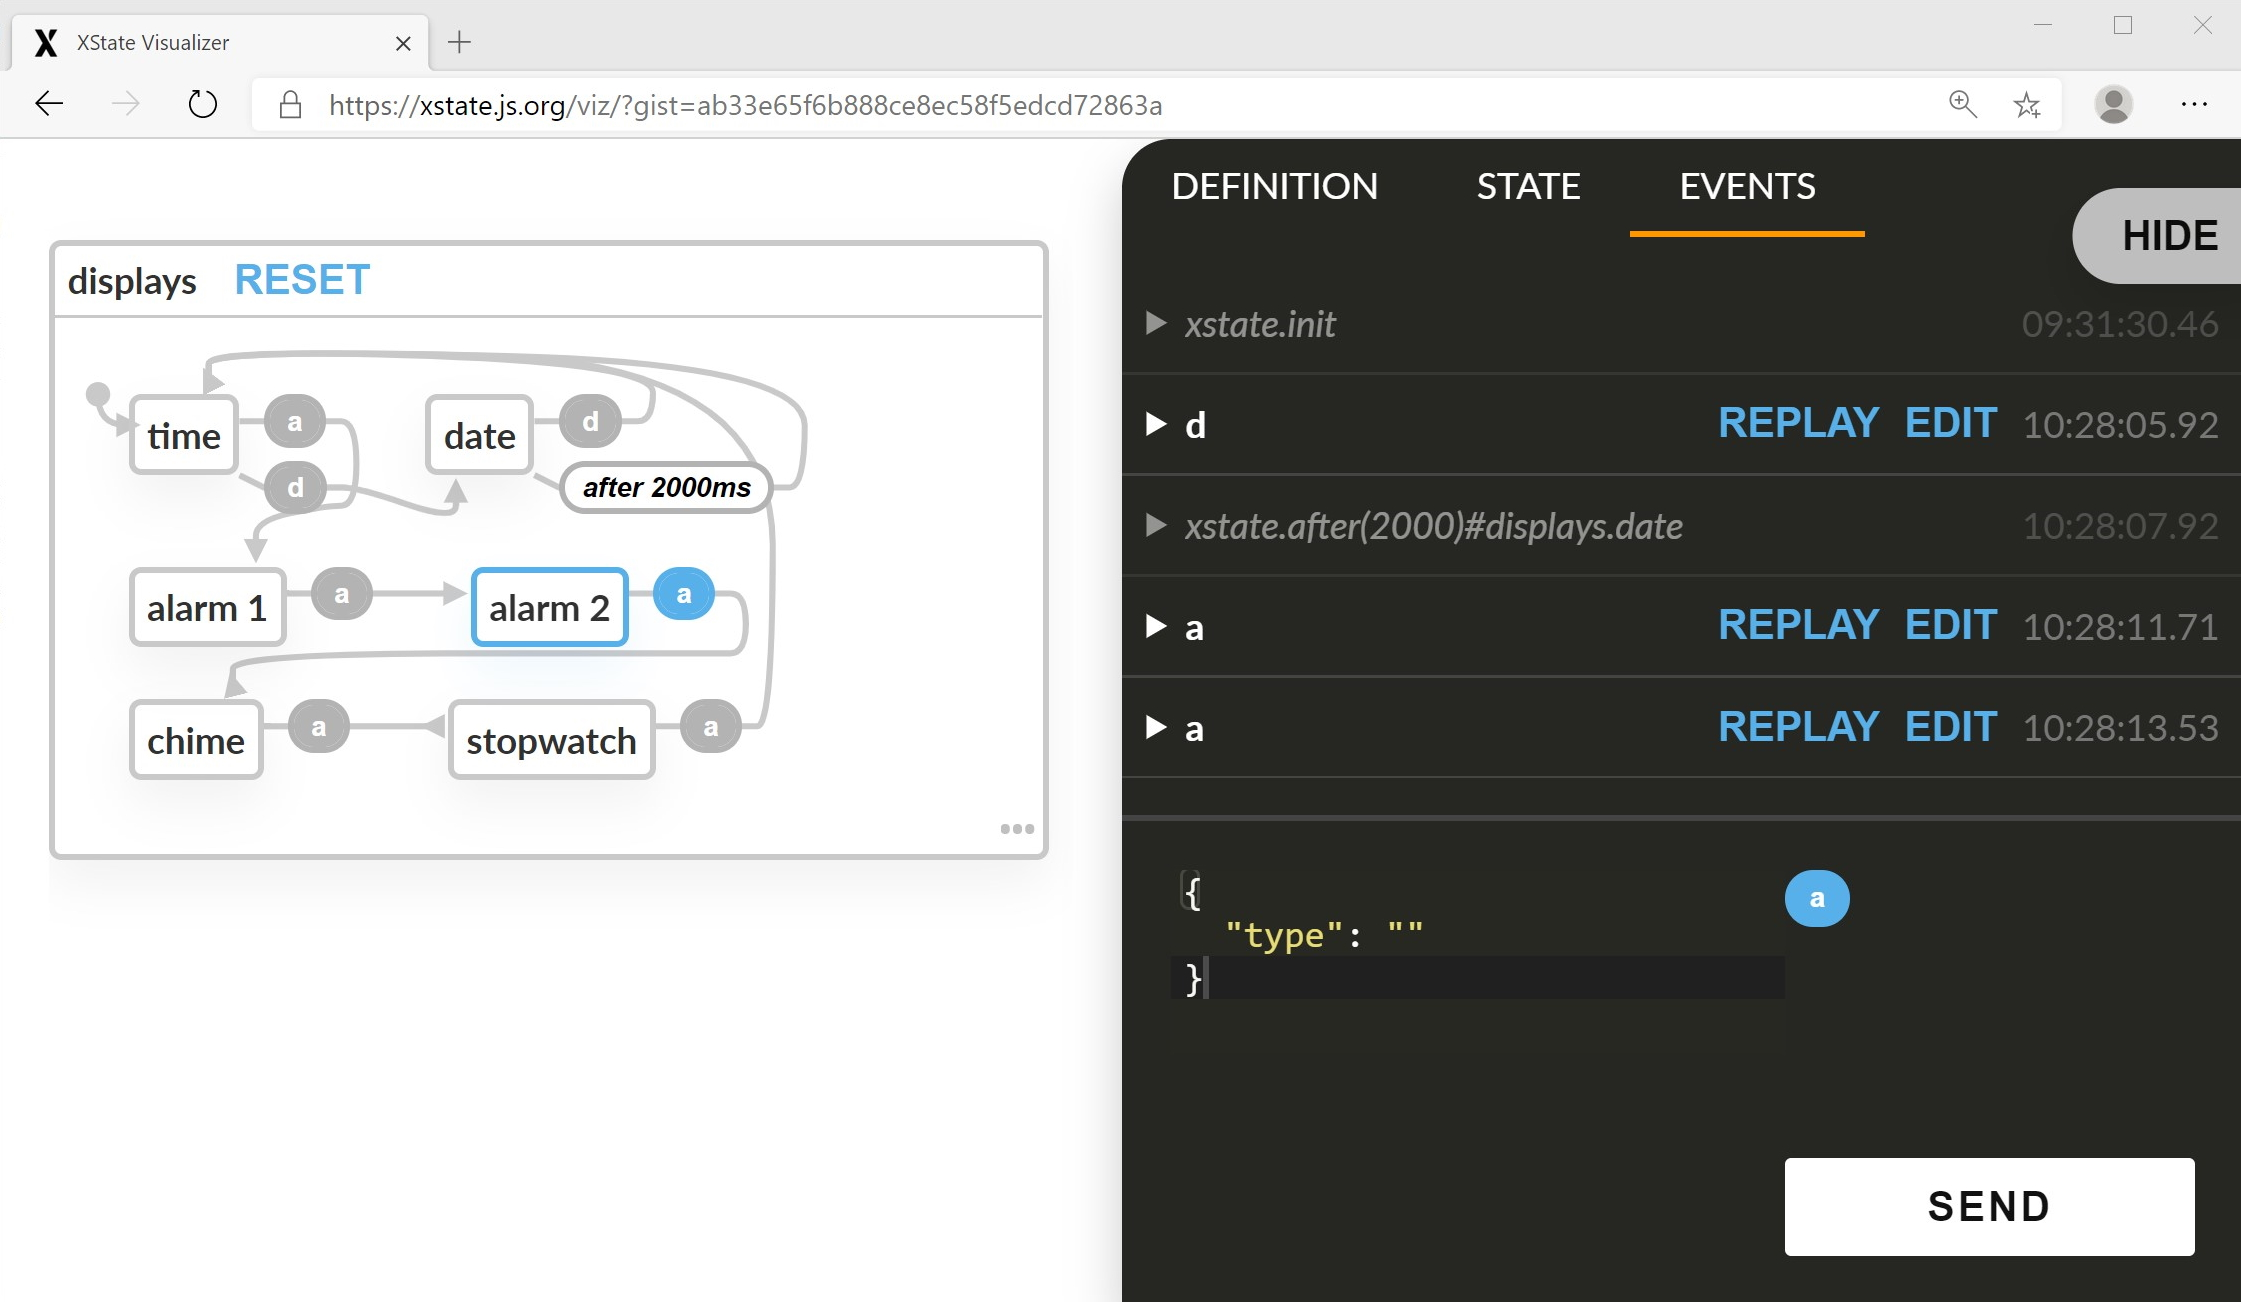
\includegraphics[width=0.9\textwidth]{images/xstate-simulation}
\caption{Simulating Statecharts using the XState Visualizer}
\label{fig:xstate-simulation}
\end{figure}
Despite differences in the notation, the statechart on the left\footnote{\url{https://xstate.js.org/viz/?gist=ab33e65f6b888ce8ec58f5edcd72863a}} is identical to \cref{fig:statecharts-example}.
On the right side there is an overview of the occurred events over time, the currently active state is highlighted directly in the statechart.
Events can be raised by clicking on the event names directly in the statechart.
Looking at the event log one can reconstruct why the currently active state is \emph{alarm 2}.
After initialization the statechart was in the state \emph{time}. Sending the event \emph{d} sent the statechart into state \emph{date}, after 2 seconds it transitioned back into \emph{time}.
Sending the event \emph{a} twice, it first transitioned into \emph{alarm 1} and then continued into \emph{alarm 2}.
Creating this mental model of the system, one can simply play around with this interactive visualization immensely reducing the cognitive effort of sharing the underlying mental model \autocite{dutke_mentale_1994}.

% - executability
% - Haskell deferring errors to runtime \verb|-XHoles|
\chapter{Discussion}
\todo{that's new}
\label{chap:discussion}
\epigraph{``One way to define `programming' is as the process of transforming a mental plan of desired actions for a computer into a representation that can be understood by the computer.''}{\textit{Jean-Michel Hoc}}
As Jean-Michel Hoc put it into words, a programmer's main task is explanation.
Before something can be explained, it must be understood deeply, also called the process of theory building as \textcite{naur_programming_1985} observed, a predominantly psychological process.
The major difficulty in interdisciplinary research is finding the sweet spot between the academic fields under research.
This thesis is neither intended to generate groundbreaking findings in psychology, nor in software engineering, much more it should be a propositional thesis, it should be food for thought, proposing ideas that may lead to new fields of research.

\textcite[10]{sheldon_software_2000} put the author's intention for starting the research on the psychological aspects of statecharts into words: "Consequently, this approach can help to avoid the waste problem that results in redevelopment effort from incorrectly specified products."
The findings in the thesis definitely highlight the similarities between mental models and statecharts extended by hole-driven development.
Whether the ideas presented in this thesis are applicable to reality, needs to be investigated in future research due to the nature of this thesis being a literature research.

One might ask why statecharts are not standard in reactive application development.
\textcite{harel_statecharts_2007} himself reflected on this topic concluding, that the official semantics of statecharts were specified way too late which lead to the development of conflicting semantics that fractured the community.
Additionally a lack of tools and learning resources might be the reason for the low adoption of such a promising concept, indicating the irony that a model suitable for transferring mental models failed at transferring itself.
\textcite{breen_statecharts_2004} published a critical view on statecharts stating that they might be too complex, suggesting that some features could be removed without losing necessary expressiveness.
Regarding the topic of requirements analysis \textcite{glinz_statecharts_2002} examined how statecharts could be used as requirements models stating that: "I have concentrated on requirements models only. The applicability and usability of the proposed statechart variant for other purposes, in particular for architecture and detailed design remains to be investigated." \autocite[5]{glinz_statecharts_2002}
The usability of statecharts might as well be a really interesting research topic especially with groundbreaking papers released long after the formalism of statecharts such as ``The `Physics' of Notations'' \autocite{moody_physics_2009}.

Further research topics might be: utilizing the model aspect of statecharts to create real evolutionary prototypes (targeted at computer scientists), the psychology of thinking in states and how this is related to preventing failures (targeted at psychologists) or adding the concept of literate programming (conveying mental models even better, [\textcite{knuth_literate_1984}]) to the ideas presented in this thesis.


% - [Matthew Frederick - three levels of knowing](https://twitter.com/Kpaxs/status/1115633791966511109)



% \section{Further Implications}
% \subsection{Building Prototypes}
% \subsection{Thinking in States/Preventing Errors}
% \subsection{Analyzing Requirements}
% - \autocite{leveson_experiences_1991}

% \section{Literate Programming}
%- Human-Computer vs. Human-Human Interaction
%\label{sub:literate-programming}
%- Communicating Mental Models \autocite[275]{kitchenham_research_1990}
%- \url{https://en.wikipedia.org/wiki/Literate_programming}
%- \autocite[235]{naur_programming_1985}
%- METAPHORS WE COMPUTE BY - Alvaro Videla
%  - \url{https://alvaro-videla.com/2017/01/metaphors-we-code-by.html}
%  - \url{https://hooktube.com/watch?v=hKOzJWNRBWA&feature=youtu.be}

\listoffigures
\printbibliography

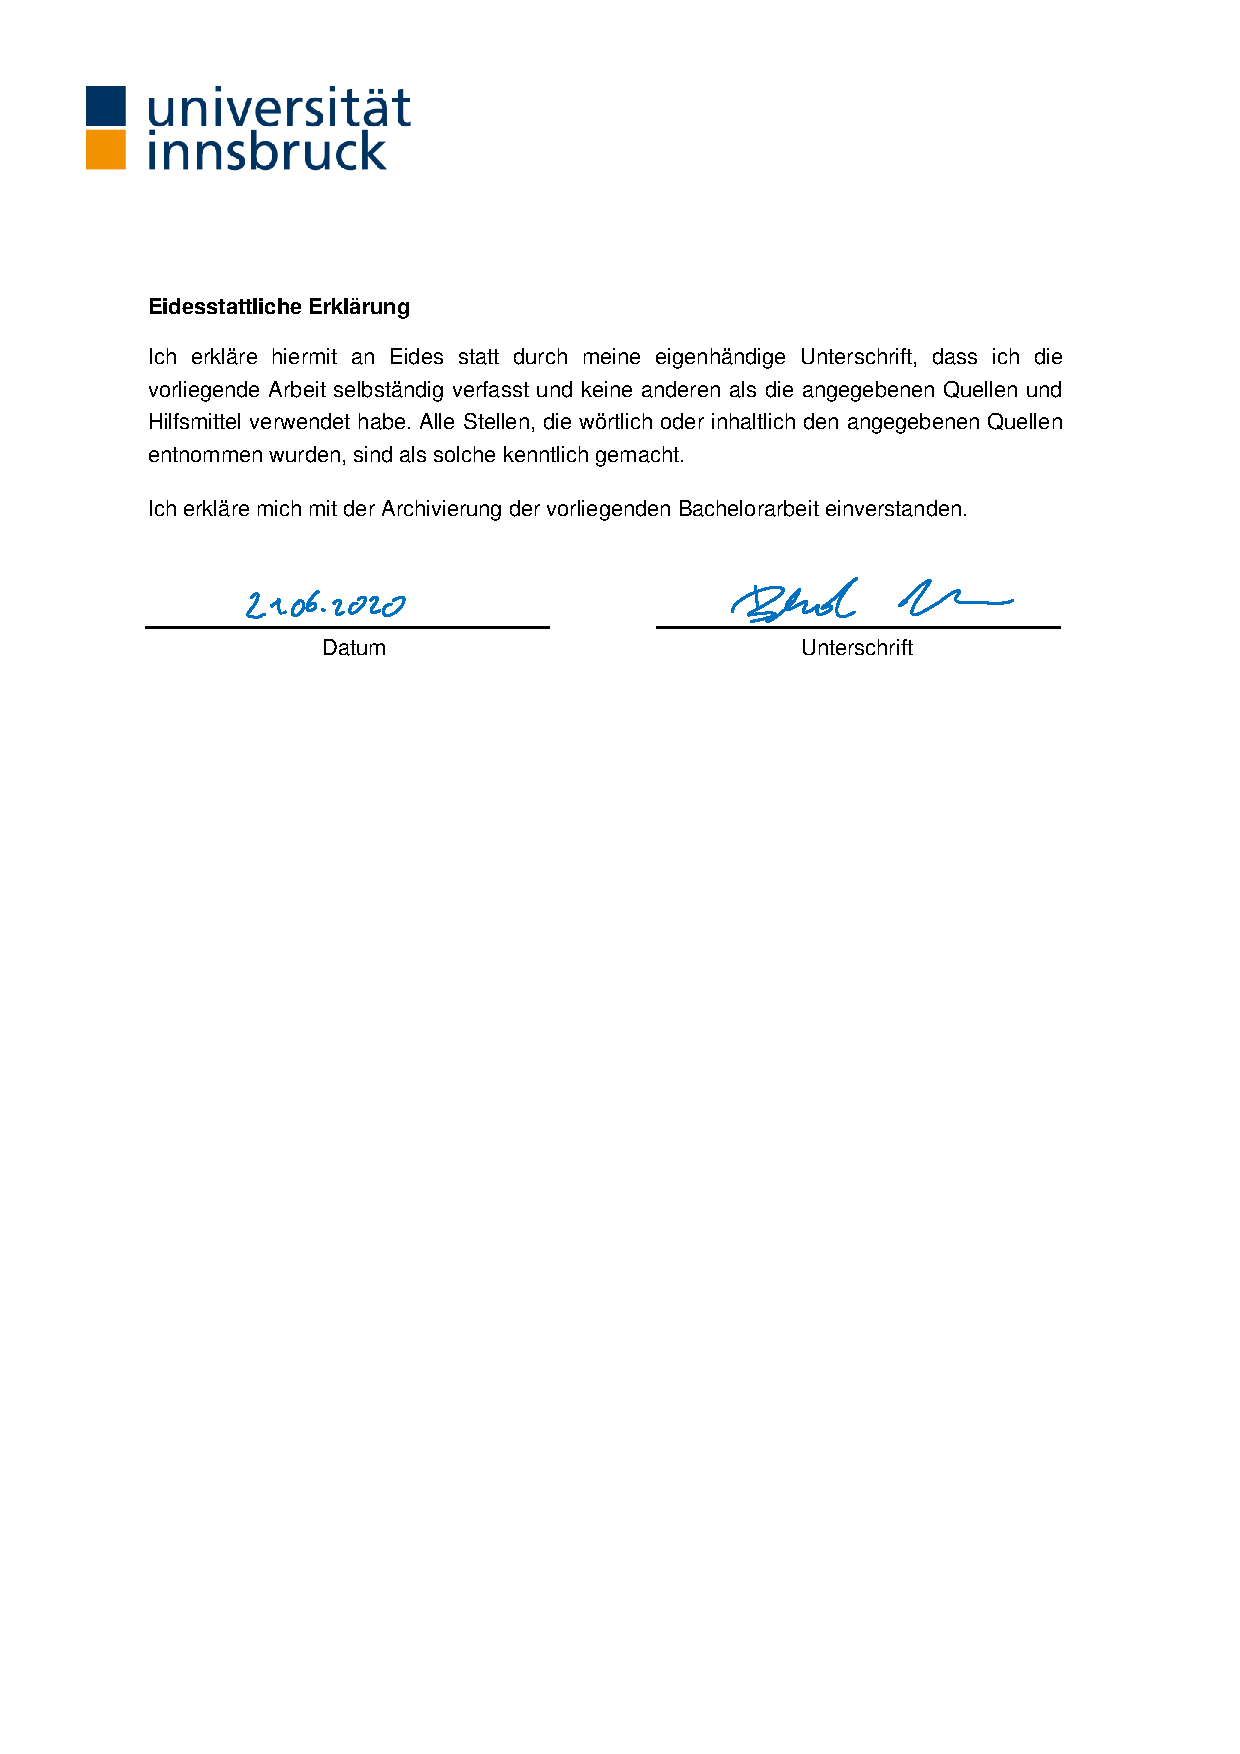
\includepdf[pages=-]{formal-parts/eidesstattliche-erklaerung}

\end{document}